\documentclass{sigchi}

% Use this section to set the ACM copyright statement (e.g. for
% preprints).  Consult the conference website for the camera-ready
% copyright statement.

% Copyright
\CopyrightYear{2017}
%\setcopyright{acmcopyright}
\setcopyright{acmlicensed}
%\setcopyright{rightsretained}
%\setcopyright{usgov}
%\setcopyright{usgovmixed}
%\setcopyright{cagov}
%\setcopyright{cagovmixed}
% DOI
%\doi{http://dx.doi.org/10.475/123_4}
% ISBN
%\isbn{123-4567-24-567/08/06}
%Conference
%\conferenceinfo{CHI'16,}{May 07--12, 2016, San Jose, CA, USA}
%Price
%\acmPrice{\$15.00}

% Use this command to override the default ACM copyright statement
% (e.g. for preprints).  Consult the conference website for the
% camera-ready copyright statement.

%% HOW TO OVERRIDE THE DEFAULT COPYRIGHT STRIP --
%% Please note you need to make sure the copy for your specific
%% license is used here!
% \toappear{
% Permission to make digital or hard copies of all or part of this work
% for personal or classroom use is granted without fee provided that
% copies are not made or distributed for profit or commercial advantage
% and that copies bear this notice and the full citation on the first
% page. Copyrights for components of this work owned by others than ACM
% must be honored. Abstracting with credit is permitted. To copy
% otherwise, or republish, to post on servers or to redistribute to
% lists, requires prior specific permission and/or a fee. Request
% permissions from \href{mailto:Permissions@acm.org}{Permissions@acm.org}. \\
% \emph{CHI '16},  May 07--12, 2016, San Jose, CA, USA \\
% ACM xxx-x-xxxx-xxxx-x/xx/xx\ldots \$15.00 \\
% DOI: \url{http://dx.doi.org/xx.xxxx/xxxxxxx.xxxxxxx}
% }

% Arabic page numbers for submission.  Remove this line to eliminate
% page numbers for the camera ready copy
% \pagenumbering{arabic}

% Load basic packages
\usepackage{balance}       % to better equalize the last page
\usepackage{graphics}      % for EPS, load graphicx instead 
\usepackage[T1]{fontenc}   % for umlauts and other diaeresis
\usepackage{txfonts}
\usepackage{mathptmx}
\usepackage[pdflang={en-US},pdftex]{hyperref}
\usepackage{color}
\usepackage{booktabs}
\usepackage{textcomp}

\usepackage[ngerman]{babel}

% Some optional stuff you might like/need.
\usepackage{microtype}        % Improved Tracking and Kerning
% \usepackage[all]{hypcap}    % Fixes bug in hyperref caption linking
\usepackage{ccicons}          % Cite your images correctly!
% \usepackage[utf8]{inputenc} % for a UTF8 editor only

% If you want to use todo notes, marginpars etc. during creation of
% your draft document, you have to enable the "chi_draft" option for
% the document class. To do this, change the very first line to:
% "\documentclass[chi_draft]{sigchi}". You can then place todo notes
% by using the "\todo{...}"  command. Make sure to disable the draft
% option again before submitting your final document.
\usepackage{todonotes}

% Paper metadata (use plain text, for PDF inclusion and later
% re-using, if desired).  Use \emtpyauthor when submitting for review
% so you remain anonymous.
\def\plaintitle{Smart Shelf: Project Proposal}
\def\plainauthor{Kevin Denk, Md. Abdul Kadir, Atika Akmal}
\def\emptyauthor{}
\def\plainkeywords{Smart Fabrication, Smart, Shelf, HCI, Physical Computing}
\def\plaingeneralterms{Project Proposal}

% llt: Define a global style for URLs, rather that the default one
\makeatletter
\def\url@leostyle{%
  \@ifundefined{selectfont}{
    \def\UrlFont{\sf}
  }{
    \def\UrlFont{\small\bf\ttfamily}
  }}
\makeatother
\urlstyle{leo}

% To make various LaTeX processors do the right thing with page size.
\def\pprw{8.5in}
\def\pprh{11in}
\special{papersize=\pprw,\pprh}
\setlength{\paperwidth}{\pprw}
\setlength{\paperheight}{\pprh}
\setlength{\pdfpagewidth}{\pprw}
\setlength{\pdfpageheight}{\pprh}

% Make sure hyperref comes last of your loaded packages, to give it a
% fighting chance of not being over-written, since its job is to
% redefine many LaTeX commands.
\definecolor{linkColor}{RGB}{6,125,233}
\hypersetup{%
  pdftitle={\plaintitle},
% Use \plainauthor for final version.
%  pdfauthor={\plainauthor},
  pdfauthor={\emptyauthor},
  pdfkeywords={\plainkeywords},
  pdfdisplaydoctitle=true, % For Accessibility
  bookmarksnumbered,
  pdfstartview={FitH},
  colorlinks,
  citecolor=black,
  filecolor=black,
  linkcolor=black,
  urlcolor=linkColor,
  breaklinks=true,
  hypertexnames=false
}

% create a shortcut to typeset table headings
% \newcommand\tabhead[1]{\small\textbf{#1}}

% End of preamble. Here it comes the document.
\begin{document}

\title{\plaintitle}

\numberofauthors{3}
\author{%
	\alignauthor{Md. Abdul Kadir\\
		\affaddr{Saarland University}\\
		\affaddr{Saarbr{\"u}cken, Germany}\\
		\email{maktareq@gmail.com}}\\
  \alignauthor{Kevin Denk\\
    \affaddr{Saarland University}\\
    \affaddr{Saarbr{\"u}cken, Germany}\\
    \email{s8kedenk@stud.uni-saarland.de}}\\
  \alignauthor{Atika Akmal\\
    \affaddr{Saarland University}\\
    \affaddr{Saarbr{\"u}cken, Germany}\\
    \email{atikaakmal19@gmail.com}}\\
}

\maketitle

\begin{abstract}
  We are on the apex of interaction technology integration with every analogue system that is used in our daily life. Working in big lab with lot of consumable equipments or finding a product in a supermarket is really a big deal. It's really hard for a person to find an object from a gigantic shelf. Also, it's hard to keep supply continuous of consumables by checking every individual slots.Sometime, it's impossible. To ease the hard work of management and user we introduce Smart Shelf that will bring smoothest interaction between shelf and human.Here, we present the overall framework, related work and the time line to implement a prototype of Smart Shelf. 
\end{abstract}

\category{H.5.m.}{Information Interfaces and Presentation
  }{Human Computer Interaction}

\keywords{\plainkeywords}

\section{Introduction}
Today the word smart is almost everywhere. 
There are smart homes and smart fabrications. 


\section{Problem}
Most people when they hear about a shelf they think about their bookshelf or some shelves in the kitchen. 
Almost everyone who have a bookshelf searched at least one time in his/her life for a book in it and wished to have a guideline how to find it the fastest way. 
Imagine big shelves with a lot of small drawers. 
Every drawer is only labelled with a small name which describes what is in that drawer. 
Searching for items in these shelves can be hard and cost a lot of time. 
An additional scenario is if you apply this concept to big warehouses with hundreds of shelves and more drawers or places where you can place items. 
Finding in such a warehouse an item can be still harder. 

Especially if you use shelves to store for example electronic components the next problem appears if you finally found the correct drawer with the searched component. 
The drawer is empty and no one ordered supplies. 
This is not only annoying, also the productivity of team sinks. 
Maybe the team or colleague can not finish work because they need that component that is not in stock currently. 
\\
\\
Not only warehouses or storage rooms with shelves have those problems with the inefficiency in finding items or the premise if one item is out of stock. 
The same problems appear in retail. 
Customer which can't find their favourite product in a shop are unsatisfied. 
Maybe they go to another shop and from that moment go directly to that other shop. 
This problem can also be tackled with smart shelves. 
The shelf itself could detect if some products in it are only available in a small amount. 
In this case the shelf could order new products or at least send an information to an operator who can order supplies. 
With this strategy there will be no more empty shelves in shops and customers can find their favourite product all the time. 

Smart Shelf should be a solution for these problems. 
It could observe the amount of items in itself, help people to find products and also order supplies if the amount of items is low. 
Furthermore, if you have a shelf with sensitive items or secrete documents, one can think about to restrict the access to some drawers. 
Drawers could be locked and only with scanning the appropriate QR-code on the drawer the drawer opens if the user is trustful. 


\section{Related Work}

There are several development work happened last few year in human computer interaction(HCI), home automation and embedded technology. A big set of these work is giving intelligence to rigid objects and allow human to communicate with them and vice-versa by applying noble HCI techniques. Moreover, post-WIMP devices also offer some features that can be integrate with the modern computer technology development(Ubiquitous computing). However, this post-WIMP GUI concept only applicable if there is a metaphor available in digital or analogue world. For example, searching the meaning of a word in digital dictionary(e.g:Smart phone dictionary). We want explain decent amount of successful research work that overlap at least in certain area with our Smart Shelf framework; However, there is no implementation or ground work fully overlap with our concept. A technical definition of our project is "Combining different interaction technique to innovate a device that follow the guideline of ubiquitous computing".The most related topic that are already known by design community are: QR code for presenting information, Automatic amount calculation, Controlling device.    
\subsection{QR code for presenting information}
Now a days application of QR code become very popular and common due to the smart phone technology. Now people don't need to type search. Pressing a key is enough to get information based on QR code. A very innovative application is using QR code in library management. In a case study ` `Application of QR Code Technology in providing Library and Information Services in Academic Libraries'' by  Sandeep
Kumar Pathak showed that important information can be presented by QR code and user can easily get all those information by scanning QR code. 
We are implying this idea in to completely different perspective. In our case every drawer will have individual QR code. Each code will represent individual information about items stored in the drawer. 
\subsection{Automatic amount calculation}
One major objective our implementation is representing empty or not empty drawer. As it's a very ground level work of many automation project, there are many project information available regarding weight measurement. However, in our project we are counting the objects based on the overall weight. We don't see this sort of work is not very common to automation community.Although, the most related work to that sub task is counting weight based on resistive sensor. An example of this work presented in $circuitdigest.com$:Arduino Weight Measurement using Load Cell and HX711 Module. Here they use Load Cell, but we will use resistive load sensor to calculate the weight signal.Also, their project does not include counting.
\subsection{Controlling Device}
The most important human to machine interaction task in this project is giving command to the system. There are several way to build up the this interaction system:one could be developing from scratch and another is building up over existing individual system. It's very common in Internet of Things (IoT) community to to use a smart phone for controlling a electronic system.For example there are lot of projects that use android devices for home automation. However, Our approach is similar but objective is completely different.
\\
\\
We see there are many existing work happened in granular level, but here we are bringing these granular ideas to build completely a new noble system.

\section{Approach}
The Smart Shelf is able to recognize low storage of items. 
Additionally, it should support user to find the search item in a shelf and show the location of it. 
This section will explain further details of the Smart Shelf. 
A description of what features the shelf will provide and how it works will be covered in this section. 
This work will provide a prototype of a smart shelf which is representative for a bigger application. 
For the prototype a shelf similar to the shelf in figure \ref{fig:example_shelf} will be used. 
%
\begin{figure}
	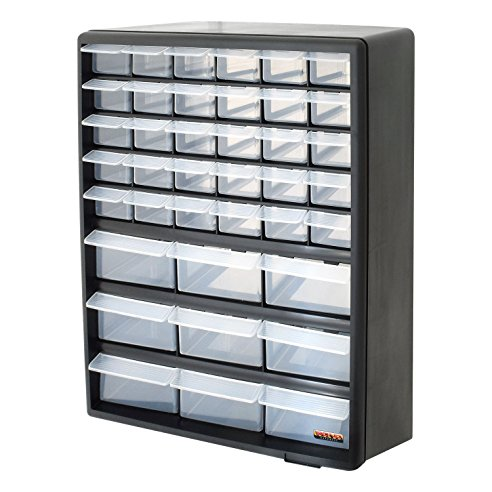
\includegraphics[width=0.9\columnwidth]{figures/example-prototype-shelf}
	\caption{Example for used Shelf as prototype.}~\label{fig:example_shelf}
\end{figure}
%
\\
\\
The Smart Shelf contains drawers with several products/items. 
With a smart phone app or another device the user can search for a specific product which may contained in the shelf. 
Is the item contained in the shelf, a light mounted at the drawer which contains the item, will switch on. 
This indicates where the user can get the item.
There is no need to scan the whole shelf for the searched item. 
The amount of items in one drawer can be measured with the weight of one item. 
With this information the Smart Shelf can display the amount of items in a drawer and also if it is empty. 
An empty drawer is indicated with a red light mounted on the drawer. 

To design the Smart Shelf \glqq{}smart\grqq{} it uses the information of the amount of items for trigger a so called \textit{low stock alarm}. 
This results in emails send to configured addresses. 
The receiver can subsequently order supplies of that item. 


\subsection{Determine amount of Items}



\subsection{Assumptions}
To realize this prototype we assume some preconditions which are listed in the following.
\\
\\
All items in the shelf either without packaging or with packaging. 
There will be no drawer where items be mixed. 
Furthermore, at any time there is only one sort of items in one drawer. 
Every drawer contains a different item. 


\subsection{Inputs}
The system prototype needs different inputs. 
These are listed in the following. 
%
\begin{itemize}
	\item Search word for an item. 
	\item Weights of the items in a corresponding drawer. 
	\item Scanned QR-code on the drawer to get more information about the containing item. 
\end{itemize}


\subsection{Outputs}
The outputs of the system are the following. 
%
\begin{itemize}
	\item Green lights on the drawer which indicates in what drawer the searched item can be found. 
	\item Red lights on the drawer which indicates if the item contained in that drawer is out of stock. 
	\item Email to configured email addresses as \glqq{}low stock alarm\grqq{} to signal if there is only a low amount of items in a drawer or the item is out of stock. 
	\item By scanning the QR-code the app shows information about the item contained in the scanned drawer. 
\end{itemize}


\subsection{User Interaction}


\section{Expected Results}
This section describes the different features the prototype of the Smart Shelf will provide. 
User are able to search with keywords for specific items may contained in the shelf. 
If the item is there the appropriate drawer will be highlighted with a green light. 
If there is only a low amount of itmes left in a drawer, a so called \textit{low stock alarm} will be triggered. 
This results in an email to configured email addresses. 
In further iterations this can end in an automatic ordering. 
So that all items in the shelf will be always available. 
Is a item out of stock the appropriate drawer is marked with a red light. 

The QR-Codes mounted on every drawer can be scanned by a smart phone app. 
This app will display information about the item contained in the scanned drawer, order information and amount of items left. 


\section{Time Plan}



\section{Conclusion}


\section{Acknowledgements}

Sample text: We thank all the volunteers, and all publications support
and staff, who wrote and provided helpful comments on previous
versions of this document. Authors 1, 2, and 3 gratefully acknowledge
the grant from NSF (\#1234--2012--ABC). \textit{This whole paragraph is
  just an example.}

% Balancing columns in a ref list is a bit of a pain because you
% either use a hack like flushend or balance, or manually insert
% a column break.  http://www.tex.ac.uk/cgi-bin/texfaq2html?label=balance
% multicols doesn't work because we're already in two-column mode,
% and flushend isn't awesome, so I choose balance.  See this
% for more info: http://cs.brown.edu/system/software/latex/doc/balance.pdf
%
% Note that in a perfect world balance wants to be in the first
% column of the last page.
%
% If balance doesn't work for you, you can remove that and
% hard-code a column break into the bbl file right before you
% submit:
%
% http://stackoverflow.com/questions/2149854/how-to-manually-equalize-columns-
% in-an-ieee-paper-if-using-bibtex
%
% Or, just remove \balance and give up on balancing the last page.
%
\balance{}

% BALANCE COLUMNS
\balance{}

% REFERENCES FORMAT
% References must be the same font size as other body text.
\bibliographystyle{SIGCHI-Reference-Format}
\bibliography{sample}



\end{document}

%%% Local Variables:
%%% mode: latex
%%% TeX-master: t
%%% End:
